\NeedsTeXFormat{LaTeX2e}[1995/12/01]

\documentclass[11pt,twoside,onecolumn,a4paper,openright,notitlepage]{book}[2001/04/21]
\usepackage[dvips]{graphicx}
\usepackage{marvosym}
\pagestyle{empty}

\usepackage{epsfig}
\usepackage{amssymb}
\usepackage{array}
\usepackage{textcomp}
\usepackage{longtable}
\usepackage[pdftex, colorlinks=true, urlcolor=black]{hyperref}

\addtolength{\hoffset}{-1.0cm}
\addtolength{\textwidth}{2.0cm}
\setlength{\oddsidemargin}{50pt}
\setlength{\evensidemargin}{50pt}

\usepackage{fancyhdr}
\pagestyle{fancy}
\renewcommand{\chaptermark}[1]{%
 \markboth{\thechapter.\ #1}{}}
%\fancyhead[LO, RE]{version 0.22 (rc1)}
\fancyhead[LE, RO]{\it pyWordom User's Guide}

\fancyfoot[C]{\thepage}

\makeatletter
\def\@makeschapterhead#1{%
  \vspace*{-00\p@}%
  {\parindent \z@ \raggedright
    \normalfont
    \interlinepenalty\@M
    \Huge \bfseries  #1\par\nobreak
    \vskip 40\p@
  }}
\makeatother

\hypersetup{%
  pdfauthor={Michele Seeber},%
  pdftitle={Wordom User's Guide},%
  pdfsubject={Manual for the Wordom molecular structures and dynamics analysis program},
  pdfkeywords={wordom, molecule, dynamics, analysis}
}
\setcounter{tocdepth}{4}
\hyphenation{PROGRESSIVE mseeber}
\pdfinfo{
  /Author (Michele Seeber)
  /Title  (Wordom Users' Guide)
  /CreationDate (D:20140724180000)
  /Subject (The Users' Guide for Wordom, the friendly molecular structure analysis and manipulation tool)
  /Keywords (Wordom, molecule, analysis)
}

\begin{document}

\pagenumbering{roman}
% ##################### Ad Hoc Built Title Page ##################### %

\begin{titlepage}
\begin{center}
\rule[1cm]{15cm}{0.05cm}
%\vspace{4.0cm}
\bfseries {\huge PyWordom User's Guide}\\ \vspace{0.4cm}
          {\large w-version 0.23-rc1}\\ \vspace{0.2cm}
          {\large July 2014}
\rule[-0.5cm]{15cm}{0.051cm}

\vspace{2.25cm}
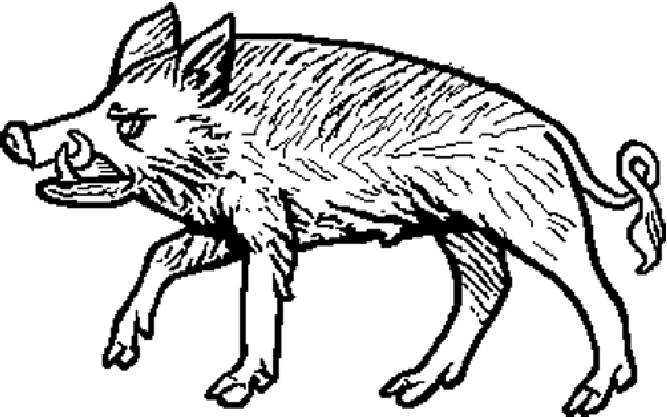
\includegraphics[scale=0.75]{images/wlogo.pdf}
\end{center}
\vspace{2.25cm}
%
\noindent\textbf{\large Developers}: Michele Seeber
\vspace{0.3cm}

\noindent\textbf{\large License}: GPL
\vspace{0.3cm}

\noindent\textbf{\large URL}: \url{http://wordom.sf.net/}
\vspace{0.3cm}

\noindent\textbf{\large Mantainer}: \href{mailto:mseeber@unimore.it}{mseeber@unimore.it}
\vspace{0.3cm}

\noindent\textbf{\large Description}: pyWordom is a python module derived from the Wordom program, automatically generated with the SWIG tool. 
\end{titlepage}
\thispagestyle{plain}
\cleardoublepage

% ##################### ####################### ##################### %
\tableofcontents
\clearpage

\pagenumbering{arabic}




\chapter{Introduction}
The basic IO functions of Wordom have been wrapped with the SWIG\cite{Beazley:SWIG} tool into a python\cite{python} module.\\
\section{Installation}
Since the pywordom module is not pure python but has a compiled C core it must be recompiled, too. To recompile just go to the sources directory and type:
\begin{verbatim}
python setup.py build
\end{verbatim}
Then, as root, run the command:
\begin{verbatim}
python setup.py install
\end{verbatim}
This will install the wordom python module in system directories. The {\em import wordom} line in a python script will include the wordom module.
\begin{verbatim}
#!/bin/env python
import wordom as wrd
\end{verbatim}


\chapter{Usage}
The {\em wordom} python module allows simple python scripts to access data in the pdb, crd, dcd and xtc formats. Most of the available functionalities are provided through the {\em molecule}, {\em trajectory}, {\em coordinates} and {\em selection} objects:

\section{Classes}

\subsection{Molecule}
The Molecule class ( wordom.Molecule ) contains all the informations read from molecule files such as pdb and crd files. These data are further processed and a molecule$\rightarrow{}$chains$\rightarrow{}$segments$\rightarrow{}$residues$\rightarrow{}$atoms tree is built.
\subsubsection{members}
nato: number of atoms\\
nRes: number of residues\\
nSeg: number of segments\\
nChain: number of chains\\
chains: list of chains\\
\subsubsection{methods}
read : read molecule file into instance ( mol1.read("mymol.pdb") )\\
write : write instance content to a file ( mol1.write("output.pdb")\\
\subsubsection{iterator}
iterating on a molecule will return pointers to chain objects (see below).

\subsection{Chain}
The Chain class describes chains, a subdivision of a molecule.

\subsection{Segment}
The Segment class describes segments, a subdivision of a molecule and collection of residues, usually continuous. Segments can be seen as a subdivision of chains. Not all molecular file formats account for both chains and segments (\emph{eg} crd files do not have chains).

\subsection{Residue}
The Residue class describes residues, usually an aminoacid.

\subsection{Atom}
The Atom class describes atoms, the smallest unit in a description of a molecule in the usual molecular mechanics workframe.

\subsection{Selection}
\subsubsection{members}
\subsubsection{methods}

\subsection{Trajectory}
\subsubsection{members}
\subsubsection{methods}

\section{Functions}


Create a new instance of the Molecule class:\\
mol1 = wrd.NewMolecule()

destroy a molecule instance:\\
wrd.DesMolecule(mol1)

create a selection instance:\\
sele1 = wrd.NewSele()

create a trajectory instance:\\
trj1 = wrd.NewTraj()

destroy a trajectory instance:\\
wrd.DesTrajtrj1)

create a trajectory header instance:\\
trh1 = wrd.NewTrjh()

create a coordinates set instance:\\
coor1 = wrd.NewCoor()

destroy a coordinates set instance:\\
wrd.DesCoor(coor1)

Functions and methods to play with these structure:

Accessing $nn^{th}$ coordinate inside a coordinate set:\\
coor1.x(nn)\\
coor1.y(nn)\\
coor1.z(nn)

Setting $nn^{th}$ coordinate inside a coordinate set:\\
coor1.setx(nn, xvalue)\\
coor1.sety(nn, yvalue)\\
coor1.setz(nn, zvalue)\\
coor1.setcoor(nn, xvalue, yvalue, zvalue)\\

Copying values from another coordinate set:\\
coor1.copycoor(coorset2)\\

Extract a subset of coordinates:\\
subset1 = coor.getselecoor( sele1 )\\

-\\

{\bf Example:}
\begin{verbatim}
import wordom as wrd

mymol = wrd.Molecule()
mymol.read( "./structure.pdb" )
mymol.write( "./copy.pdb" )

sele1 = mymol.select( "/CA" )
print sele1.nselatm
mymol2 = mymol.getselemol(sele1)
mymol2.write( "submol.pdb" )

\end{verbatim}

\begin{thebibliography}{10}
\addcontentsline{toc}{chapter}{Bibliography}

\bibitem{Beazley:SWIG}
D. Beazley, {\em The Simple Wrapper and Interface Generator}. Available at: \url{http://www.swig.org}

\bibitem{python}
Guido van Rossum, {\em The Python Programming Language}. Available at: \url{http://www.python.org}

\end{thebibliography}

\clearpage

% ##################### That's All Folks! ##################### %

\end{document}

